\documentclass{standalone}
\usepackage{tikz}

\begin{document}
    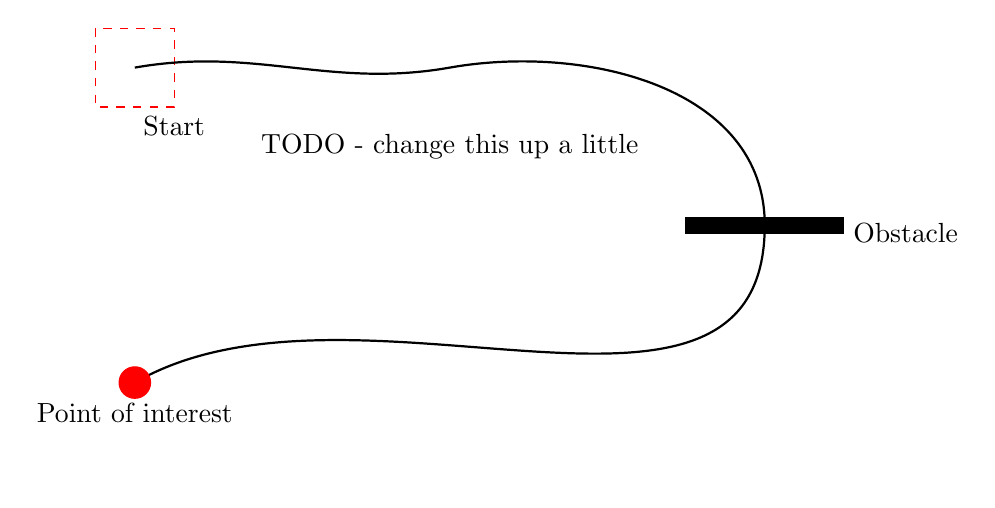
\begin{tikzpicture}
      \draw [red,dashed] (-2.5,2.5) rectangle (-1.5,1.5) node [black,below] {Start}; % Draws a rectangle
      \draw [thick] (-2,2) % Draws a line
      to [out=10,in=190] (2,2)
      to [out=10,in=90] (6,0) 
      to [out=-90,in=30] (-2,-2);    
      \draw [fill] (5,0.1) rectangle (7,-0.1) node [black,right] {Obstacle}; % Draws another rectangle
      \draw [red,fill] (-2,-2) circle [radius=0.2] node [black,below=4] {Point of interest}; % Draws a circle
      \draw node at (2,1) {TODO - change this up a little};
    \end{tikzpicture}
\end{document}